\documentclass[12pt]{article}
%\usepackage{html}
\usepackage{hyperref}
\usepackage{graphicx}
\title{CS 571\\Quiz 3 Solution}
%\addtolength{\topmargin}{-2cm}
%\addtolength{\topskip}{-2cm}
%\addtolength{\oddsidemargin}{-2cm}
%\addtolength{\evensidemargin}{-2cm}
%\addtolength{\textheight}{2cm}
%\addtolength{\textwidth}{2cm}
%\addtolength{\footskip}{-1cm}
\date{}
\begin{document}
\maketitle

\begin{flushleft}
\textbf{Oct 10}\hfill\textbf{Closed book}\\
\textbf{15 points}\hfill\textbf{Closed notes}\\

\vspace{0.5cm}

\textbf{Important Reminder}: As per the course Academic Honesty
Statement, cheating of any kind will minimally result in receiving an
F letter grade for the entire course.


\end{flushleft}

\textbf{Please ensure that you have filled-in BOTH your name and
  B-number in the bubbles on the provided grid-sheet.}

For each of the following questions, select a \textbf{single}
alternative on the grid-sheet.  

There are 7 questions with 2-points per question; there is 1-point
for submitting the quiz.

\begin{enumerate}

\item Which of the following languages over the vocabulary of
  square-brackets $\{$\verb@[@, \verb@]@$\}$ is not expressible using
  standard regular expressions?

\begin{enumerate}

\item Strings of even length.  Examples include
  the empty string, \verb@][@, \verb@[[[]@ and \verb@[[]]@.

\item Strings of even length which consist of balanced brackets.
  Examples include the empty string, \verb@[]@ and \verb@[][[]]@.

\item Strings of even length containing 2-or-more \verb@]@'s
  followed by 0-or-more \verb@[@'s.  Examples include \verb@]]@,
  \verb@]]][@ and \verb@]][[@.

\item Strings of length less-than-or-equal-to 4 which consist of
  balanced brackets. 
    Examples include the empty string, \verb@[]@ and \verb@[][]@.

\item Strings whose length is exactly 4.  Examples include \verb@]][[@,
  \verb@[[[]@ and \verb@[][]@.
  
\end{enumerate}

\textbf{Answer}: (b).

Regular expressions cannot describe arbitrary balanced constructs.
Hence (b) is not expressible.  (d) and (e) can be described by
a regex which simply enumerates all possibilities.  (a) can be
described by the regex \verb@( \[\[ | \[\] | \]\[ | \]\] )*@ and
(c) can be described by the regex \verb@(\]\])+ (\]\[)? (\[\[)*@.

\item In Javascript, \textit{hoisting} refers to:
\begin{enumerate}

\item Moving \verb@let@ declarations to the start
  of a block.

\item Moving \verb@let@ declarations to the start
  of a function.

\item Moving \verb@var@ declarations to the start
  of a block.

\item Moving \verb@var@ declarations to the start
  of a function.

\item Moving \verb@var@ declarations to the \verb@window@ object.

\end{enumerate}

\textbf{Answer}: (d).

This is the standard definition of the term \textit{hoisting} within
the Javascript community.  This behavior can surprise programmers
coming to Javascript from a language where variables have block scope.


\item What should be the value of the following Scheme expression?

\begin{verbatim}

    (length '( 1 (2 3) () () (()) ))

 \end{verbatim}


\begin{enumerate}

\item It will result in an error since the list is not a proper list.
  
\item 3

\item 4 
  
\item 5
  
\item 6
    
\end{enumerate}

\textbf{Answer}: (d).

The \verb@length@ function counts the number of top-level elements in
 the list and the list contains the following top-level elements:
\verb@1@, \verb@(2 3)@, \verb@'()@, \verb@'()@ and \verb@'(())@.  The 
last element is a 1-element list containing \verb@'()@.

\item Which of the following is the most accurate characterization of
 the semantics of \verb@cons@, \verb@car@ and \verb@cdr@ in
 Scheme?

\begin{enumerate}

\item \verb@cons@ constructs a list, \verb@car@ returns the head
of the list, \verb@cdr@ returns the tail of the list.

\item \verb@cons@ constructs a list, \verb@car@ returns the tail
of the list, \verb@cdr@ returns the head of the list.

\item \verb@cons@ constructs a pair, \verb@car@ returns the first
element of the pair, \verb@cdr@ returns the second element of the pair.

\item \verb@cons@ constructs a list, \verb@car@ returns the first
 element of the list and \verb@cdr@ returns the second element of the
 list.

\item \verb@cons@ constructs a pair, \verb@car@ returns the second
element of the pair, \verb@cdr@ returns the first element of the pair.


\end{enumerate}

\textbf{Answer}: (c).

\verb@cons@ constructs a pair, not a list (which is constructed by
\verb@list@); \verb@car@ accesses the first element of the pair
and \verb@cdr@ the second.

\item What should be the value of the following Scheme expression?

\begin{verbatim}

      (caddr '(a b c d e))

\end{verbatim}

\begin{enumerate}

  \item \verb@'b@.

  \item \verb@'c@.
    
  \item \verb@'d@.

  \item \verb@'(c d e)@

  \item \verb@'(d e)@
    
    
\end{enumerate}

\textbf{Answer}: (b).

\verb@cdr@ is \verb@'(b c d e)@; \verb@cddr@ is \verb@'(c d e)@; hence
\verb@caddr@ is \verb@'c@.


\item What should be the value of the following Scheme expression?

\begin{verbatim}

      (cdddr '(a b c d e))

\end{verbatim}

\begin{enumerate}

  \item \verb@'b@.

  \item \verb@'c@.
    
  \item \verb@'d@.

  \item \verb@'(c d e)@

  \item \verb@'(d e)@
    
\end{enumerate}
    
\textbf{Answer}: (e).

\verb@cdr@ is \verb@'(b c d e)@; \verb@cddr@ is \verb@'(c d e)@; hence
\verb@cdddr@ is \verb@'(d e)@.


\item Given the following tree structure:

  \begin{center}
    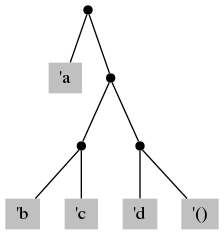
\includegraphics[height=80mm]{nest1}\\
  \end{center}

  which of the following Scheme expressions best describes the
  structure?

\begin{enumerate}

\item \verb@'(a b c d)@

\item \verb@'(a (b c) d)@

\item \verb@'(a (b . c) d)@
  
\item \verb@'(a (b c) (d ()))@


\item \verb@'(a (b c) (d . ()))@

\end{enumerate}

\textbf{Answer}: (c)

Since the right-spine of the figure ends with a \verb@'()@, the
figure represents a proper list.  The first element is \verb@'a@,
the second element is an improper list \verb@'(b . c)@ (since it does
not end with a \verb@'()@) and the last element is \verb@'d@.

\end{enumerate}

\end{document}
